\chapter{Documentación y Difusión}

Para favorecer el interés del proyecto entre los aficionados a la astronomía (y al hardware libre en general) se han emprendido diversas actividades divulgativas, como son:


\begin{itemize}
	\item Creación de una página web del proyecto.
	\item Creación de canales en redes sociales.
	\item Asistencia y presentación del proyecto en congresos astroómicos.
	\item Mantenimiento del repositorio \textbf{GitHub} con toda la información relevante del proyecto (documentación, código, diagramas...)
\end{itemize}

En las siguientes secciones se comenta más en detalle cada una de dichas actividades.


\section{Página web del proyecto}

Se diseña una página web a modo de \textbf{``landing page''} que resuma toda la información del proyecto de una forma agradable al visitante. Las caracerísticas más reseñables de dicha página web son:

\begin{itemize}
  \item Mostrar toda la información del proyecto bien catalogada y organizada en las diferentes secciones. 
 Se incluyen fotos y resumenes de algunos pasos del proyecto, lista de materiales y enlaces de descarga.

  \item Seguir diseño visual atractivo y favorecer una buena experiencia de usuario, cuidando el esquema de colores, la disposición de los elementos y su tamaño, permitiendo la navegación por el sitio de una forma cómoda e intuitiva.

  \item Diseño \textit{responsive}, asegurando que se ven todos los elementos de forma correcta en ordenadores, móviles y tabletas. 

  \item Seguir los últimos estándares HTML5, validando una correcta semántica, utilizar \textbf{metadescripciones} \cite{meta}. Con ello favorecemos  una correcta indexación por los motores de búsqueda, haciendo llegar la página al público objetivo de una forma más rápida y selectiva (uno de los principios básico de SEO \cite{seo}).
\end{itemize}

Dicha página web puede verse en \url{http://ardufocuser.info}.

\section{Canales en redes sociales}

Al comienzo del desarrollo se creó una cuenta en twitter \textbf{@ardufocusindi} con la finalidad de crear una comunidad de gente interesada en el proyecto y en otros temas relacionados.

La idea de este canal era mantener informada a la comunidad de los últimos avances del proyecto y nuevas actualizaciones así como compartir también material interesante para estar al día de los últimos avances.

Sin embargo, hay que reconocer que este intento de difusión no ha funcionado bien, probablemente por la falta de actualización así como la dificultad de publicitar algo tan específico que prácticamente solo interesa a un público objetivo muy concreto (astrónomos) sin ser el propio desarrollador un miembro de esta comunidad.


\section{Congresos Astronómicos}

Durante el proyecto he tenido la oportunidad de asistir a eventos y congresos astronómicos donde se ha promocionado el proyecto. 


\begin{itemize}
	\item \textbf{Astro-Encuentro La Sagra 2015}: Celebrado del 16 al 18 de Octubre en la localidad de la Puebla de Don Fabrique, dos días diversas actividades en el marco de la astronomía, donde tuve oportunidad de visitar el ``Observatorio Astronómico de la Sagra'' \cite{lasagra} operado, entre otros, por el Instituto de Astrofísica de Andalucía (IAA).
	
	Entre todas las actividades, por su relación con el presente proyecto, cabe destacar la ponencia de D. Nicolás Morales (investigador del Instituto de Astrofísica de Andalucía) donde realiza una demostración de una observación con telescopios manejados en remoto en tiempo real demostrando como realizan estudios de impactos en la Luna.
	
	\item \textbf{Astro-Alcala Alcalá la Real 2016}: Celebrado del 8 al 10 de Abril en la localidad de Alcalá la Real. En dicho encuentro se presentó un póster mostrando un resumen del proyecto Ardufocuser (figura~\ref{fig:posterAstroAlcala}).
	
\begin{figure}[h]
	\centering
	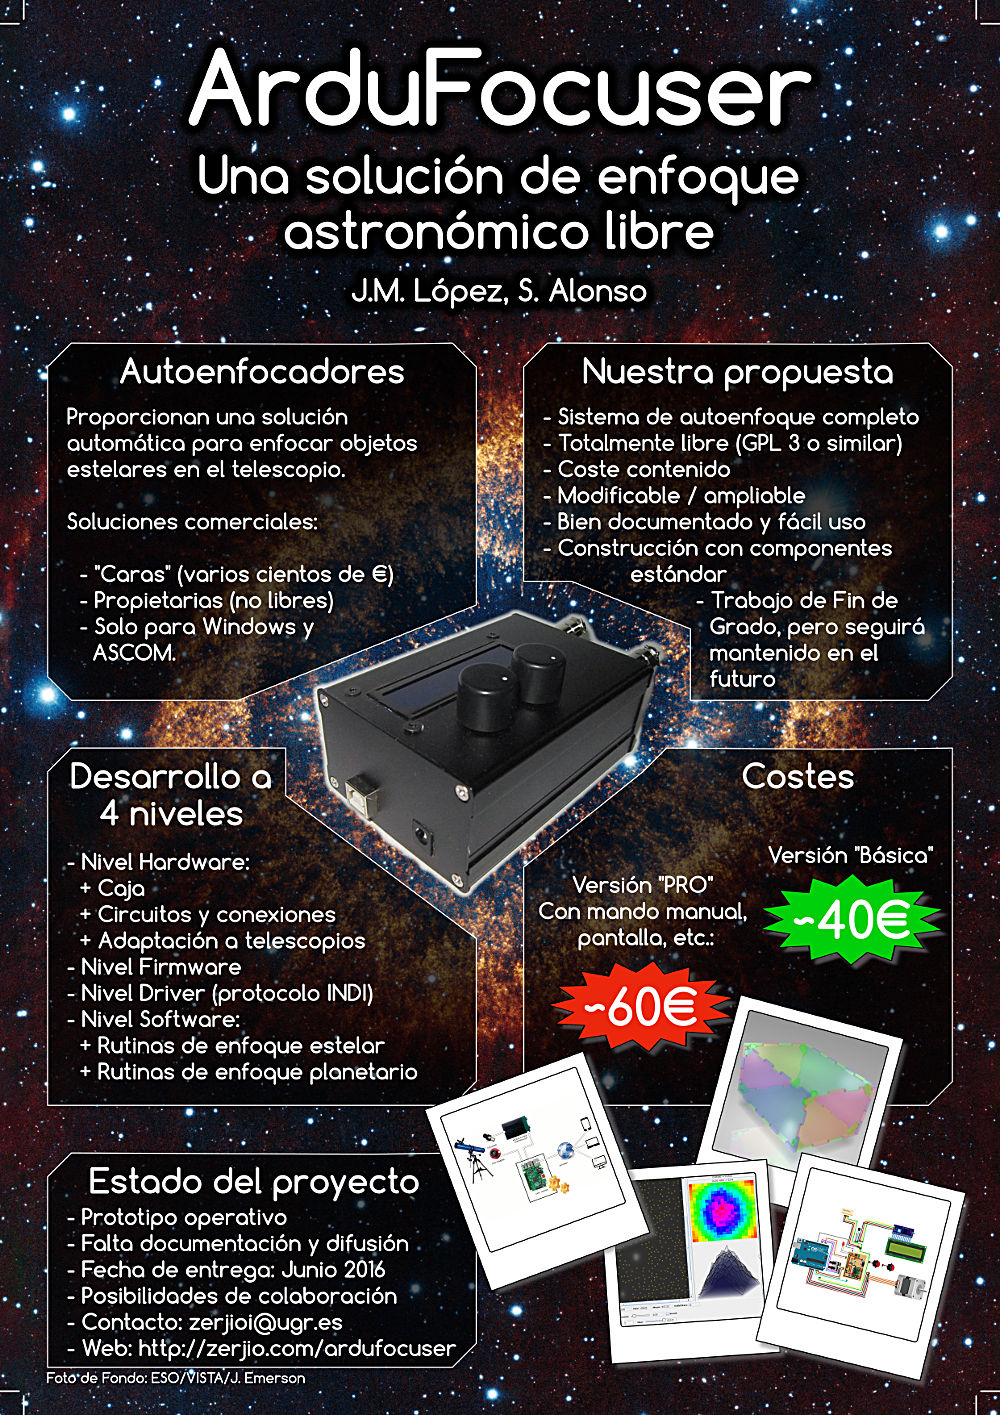
\includegraphics[width=1\linewidth]{../images/poster_Ardufocuser_AstroAlcala}
	\caption[Poster presentando el proyecto en AstroAlcalá 2016]{Poster presentando el proyecto en AstroAlcalá 2016.}
	\label{fig:posterAstroAlcala}
\end{figure}
	
	\item Presentación del proyecto \textbf{Ardufocuser} ante la SAG (Sociedad Astronómica Granadina) \cite{sag} en Febrero de 2016: En dicha presentación se mencionan a grandes rasgos las ventajas que ofrece en comparación a los productos comerciales y se comparten detalles técnicos del mismo. Varios de los asistentes mostraron mucho interés en el proyecto.
\end{itemize}
 
 
\section{Mantenimiento del repositorio GitHub}

Para el desarrollo del proyecto se ha contado con varios repositorios en Github, por comodidad uno para cada parte del proyecto. 


\begin{itemize}
	\item \textbf{Ardufocuser-firmware:} Contiene todo el código fuente del firmware que ejecuta la placa de Arduino, junto con las bibliotecas correspondientes y los scripts de pruebas. 
	\item \textbf{Ardufocuser-indidriver:} Contiene el módulo driver INDI específico para Ardufocuser, implementado en Java a partir de las especificaciones \textbf{INDIforJava}.
	\item \textbf{Ardufocuser-image-processing:} Contiene el código fuente del software de análisis de imágenes, detección de objetos y calculo de FWHM. Además cuenta con la biblioteca de manejo de imágenes FITS implementada para facilitar el trabajo.
	\item \textbf{Ardufocuser-documentations:} Contene los fuentes  \LaTeX de este mismo documento junto con las imágenes y recursos utilizados.
\end{itemize}

Utilizar GitHub me ha proporcionado grandes ventajas.

\begin{itemize}
	\item Contar con un sistema de control de versiones distribuido, con toda la potencia de \textbf{Git}.
	\item Publicar los cambios directamente y ser accesibles desde la web (se puede consultar desde un navegador web).
	\item Conectar servicio de integración continua Travis CI.
\end{itemize}

En todo momento se ha intentado cuidar el estilo y la calidad del código, añadiendo los pertinentes comentarios y utilizando nombres adecuados para nombrar variables, clases, métodos o funciones con el propósito que cualquier interesado pueda acceder al código, comprender la lógica y realizar cambios de forma fácil.  

Cualquier interesado en colaborar queda invitado a realizar \textbf{Merge Request}, indicando un resumen de la mejora o el bug que soluciona. En lo más breve se evaluará el cambio, se incorporará a la base de código y aparecerá como colaborador del proyecto.


 
